\documentclass{sig-alternate-10pt}

\usepackage{times}
\usepackage{graphics}
\usepackage{listings}
\usepackage{subfigure}
\usepackage{booktabs}
\usepackage{colortbl}
\usepackage{tabularx}
\usepackage{color}
\usepackage{xspace}
\usepackage{hyperref}    % Creates hyperlinks from ref/cite
\hypersetup{pdfstartview=FitH}
\usepackage{graphicx}    % For importing graphics
\usepackage{url}         %
\usepackage{caption}

\hypersetup{%
pdftitle={Latency Measurement and Analysis of Wide Area Networks, Data Center, and Cellular Networks}, pdfauthor={Ben Zhang, Ahir Reddy}, pdfkeywords={Internet, Latency, Measurement}, bookmarksnumbered, pdfstartview={FitH}, colorlinks,
citecolor=black, filecolor=black, linkcolor=black, urlcolor=black,
breaklinks=true,}

\renewcommand{\arraystretch}{1.2} % Space out rows in tables

\newcommand{\ml}[1]{{\color{green} {\it ML: #1}}}

% No space between bibliography items:
\let\oldthebibliography=\thebibliography
  \let\endoldthebibliography=\endthebibliography
  \renewenvironment{thebibliography}[1]{%
    \begin{oldthebibliography}{#1}%
      \setlength{\parskip}{0ex}%
      \setlength{\itemsep}{0ex}%
  }%
  {%
    \end{oldthebibliography}%
  }

%\pagenumbering{arabic}  % Arabic page numbers for submission.  Remove this line to eliminate page numbers for the camera ready copy

\begin{document}

% use this command to override the default ACM copyright statement
% (e.g. for preprints). Remove for camera ready copy.
%\toappear{Submitted for review to IPSN 2012.}
% \conferenceinfo{ConfName} {Date, Location}
% \CopyrightYear{Year} 
% \crdata{978-1-4503-1227-1/12/04} 
% \clubpenalty=10000 
% \widowpenalty = 10000


% to make various LaTeX processors do the right thing with page size
\special{papersize=8.5in,11in}
\setlength{\paperheight}{11in}
\setlength{\paperwidth}{8.5in}
\setlength{\pdfpageheight}{\paperheight}
\setlength{\pdfpagewidth}{\paperwidth}

\setlength{\textfloatsep}{13pt plus 2pt minus 1pt}

\title{Latency Measurement and Analysis of \\ Wide Area Networks, Data Center, and Cellular Networks}

\author{
{Ben Zhang, Ahir Reddy}\\
\affaddr{University of California, Berkeley}\\
%\affaddr{}\\
\email{benzh@eecs.berkeley.edu, ahirreddy@berkeley.edu}
}

\maketitle

\begin{abstract}
% Abstract for measurement project.
Understanding the current state of Internet performance is critical to both academic research and industrial systems. Though various metrics (connectivity, available bandwidth, etc.) are important to evaluate, in this project, we focus on the latency of current Internet (as of 2013) in the Wide Area Network (WAN), Data Center (DC), and Cellular Networks.

We employed the King/Turbo-King methods proposed in the literature to measure the latency between two arbitrary hosts. The correlation of latency with geographical location will allow for identification of the gap between existing network performance and the speed-of-light limit. Such data serves as the starting point for analyzing wide area network performance. As the number of services deployed in the Cloud continues to increase, how the latencies experienced by end-users are dependent on data center performance is unknown though many research efforts have been put to optimizing DC performance. We use Google Search in our case study to understand the composition of time in typical data center queries. Our final study explored cellular networks; more specifically we evaluated AT\&T's 4G-LTE network in the Bay Area. We utilized \texttt{traceroute} to test the latency of the new flat IP architecture in LTE networks.

\end{abstract}

%\category{C.2.1}{Computer-Communication Networks}{Network Architecture and Design}[Wireless communication]
%\keywords{Collection, CTP, Sensor Network, Routing}

% \category{B.0}{Hardware}{General}
% \category{B.4}{Hardware}{Input/Output \& Data Communication} 
% \category{H.4.m}{Information Systems Applications}{Miscellaneous}

% \terms{Design, Experimentation, Measurement} 
\keywords{Internet Latency, Measurement Study, King, Turbo King, Planet Lab, traceroute}

\section{Introduction}
\label{sec:introduction}

% why do measurement
The measurement of Internet has become increasingly challenging due to its complexity, large-scale, heterogeneity and variability. However, the importance is also increasing because an understanding of the performance of the Internet architecture will provide the insight necessary to design a better architecture, which is either incrementally deployable or a clean slate design. Depending on figure of interest, there exist many metrics to characterize the performance -- connectivity, available bandwidth, latency, etc. Various tools have been proposed to conduct these measurements (see Sec.\,\ref{sec:related-work} for a complete review). This work does not aim to introduce a revolutionary methodology to conduct measurements. Instead, we base our work on many existing tools and available infrastructure. We will discuss both our methodology and an analysis of the measurements we have collected.

% split up to three parts
Our work study is composed of three distinct parts: the latency in the wide-area network,  latency as experienced by end-users when interacting with the data center, and latency within cellular networks.

The goal in measuring WAN latency is to develop and understanding of how latency is related to distance. The traditional model used to calculate the latency between end-hosts is to sum propagation delay, transmission delay, queuing delay and processing delay \cite{kurose2001computer}. The propagation delay is determined by the length of cables (for wired networks), and will have the lower bound, which we refer to ``speed-of-light limit'' in this paper. The transmission delay and processing delay depend on the speed of routers (or switches) and the size of the packet. The general trend is that these delays are getting smaller. Nonetheless, queuing delay has a lot of variation depending on the traffic load; in the worst case, packets may even be dropped. In our study we aim to uncover the current state of latency in the WAN given the new and recent developments in networking hardware and software. Furthermore, we seek to make a comparison to the theoretical speed-of-light limit. In our study we have adopted the King/Turbo-King \cite{gummadi2002king, leonard2008turbo} methods and deployed measurement nodes to PlanetLab \cite{chun2003planetlab} servers located globally. In a continuous study spanning more than 10 days we have obtained approximately 5 million measurements for analysis.

In the second section of our study, we analyze cloud services and data centers. More specifically, we have chosen to perform a study of Google Search due to its popularity and Google's promise of delivering timely responses to end-users. Furthermore, we are motivated to use Google Search because of the fact that the return page from Google includes an estimate of time spent inside the data center. By inspecting the TCP trace of a query conversation, we found out that this estimated time is a fairly accurate portrayal of time spent within the data center. Because each transaction involves several rounds of data transmission, the round-trip time (RTT) will influence the overall query time. We extract Google's IP address from the packet trace using \texttt{tcpdump} and utilize \texttt{ping} to query this IP to measure the network latency. By examining this data from various vantage points (deployed to PlanetLab servers), we would partition the latency and provide insights for network optimizations.

The final aspect of our study is an analysis of cellular networks, and in particular the relatively new and growing 4G-LTE deployments. By adopting a flat IP architecture, carriers promise to reduce the network latency and decouple radio access from core network evolution. To measure the real performance of the network, we use \texttt{traceroute} to examine the latency on each hop and the routing stability within the cellular backbone.

% summarize the contribution
To summarize, we make the following contributions in this measurement study:
\begin{itemize}
\setlength{\itemsep}{1pt}
\setlength{\parskip}{0pt}
\setlength{\parsep}{0pt}
\item We present measurements of the wide-area network, the fraction of round-trip time spent within the data center, and latencies within the cellular network backbone.
\item We provide the methodology and analysis of our collected measurements.
\end{itemize}

% rest of the paper
In the rest of this paper, we will first describe the related works in Sec.\,\ref{sec:related-work}. And then we detail our measurements and analysis for WAN, DC and cellular networks in Sec.\,\ref{sec:latency-wan}, Sec.\,\ref{sec:latency-DC} and Sec.\,\ref{sec:latency-in-cellular} respectively. We discuss our experience in conducting this measurements in Sec.\,\ref{sec:discussion}. Sec.\,\ref{sec:conclusion} concludes the paper and discusses some of the future work.

% In the rest of this paper, we will first describe the related works in Sec.\,\ref{sec:related-work}. And then detail our measure methodology in Sec.\,\ref{sec:methodology}. The experiment setup is in Sec.\,\ref{sec:experiment}, which is followed by the analysis of the data in Sec.\,\ref{sec:analysis}. We then briefly discuss a few questions regarding our measurements in Sec.\,\ref{sec:discussion}. Sec.\,\ref{sec:conclusion} concludes the paper and discusses some of the future work.

%%% Local Variables: 
%%% mode: latex
%%% TeX-master: "main"
%%% End: 

\section{Related Work}
\label{sec:related-work}

%% Describe related work here.
% the following related works are more from end-host perspective.

\subsection{Tools and Infrastructures}
\label{sec:tools}

There are a number of existing tools for Internet measurement; they primarily differ in the network characteristics they measure. \texttt{ping} is the popular tool used to test reachability and measure round trip time (RTT). \texttt{traceroute} \cite{jacobson1989traceroute} and \texttt{tcptraceroute} \cite{toren2001tcptraceroute} reveal the routing path as well as the RTT. King \cite{gummadi2002king} measures the end-to-end latency of arbitrary end-hosts using recursive DNS queries. Turbo King (T-King \cite{leonard2008turbo}) proposes an alternative methodology for generating more accurate measurement results than King. \texttt{pathchar} \cite{jacobson1997pathchar} measures the hop-by-hop bandwidth and \cite{jain2002pathload} reports the available bandwidth of a path. \cite{paxson2002experiences} provides dedicated hardware for measurements that only affiliated users can access. In \cite{spring2003scriptroute}, Spring {\it et al.}, seeks to build a generic platform for ordinary users to conduct measurements from remote vantage points.

On top of these tools, many large Internet monitoring projects (such as pingER \cite{matthews2000pinger} and iPlane \cite{madhyastha2006iplane}) have been built. A number of infrastructures that serve as experimental testbeds are also available to conduct large scale measurements. Among these, GENI \cite{elliott2008geni} and PlanetLab \cite{chun2003planetlab} are two active projects.

% Furthermore, researchers are also trying to infer Internet performance and security \cite{paxson1999bro} based on measurement results (\cite{downey1999using} utilized \texttt{pathchar} tool to estimate Internet link characteristics). 

In our measurement study, we do not seek to introduce new measurement strategies or infrastructure. Instead, we derive our strategy from the King, T-King, \texttt{traceroute}, \texttt{ping}, and research-oriented infrastructure PlanetLab.

\subsection{Measurements}
\label{sec:measurements}

With the advent of cloud computing and mobile computing, it has become increasingly important to characterize the performance of the data center and mobile networks. 

Both \cite{benson2010network, kandula2009nature} analyze traffic patterns in data centers. These measurement results help in developing an understanding of the nature of traffic in an operational data center (especially for those without direct access). The measurements results have also guided many system designs. VL2 \cite{greenberg2009vl2} is one such example; the validation of Valiant Load Balancing on flow level is based on the small flow traffic pattern observed in a data center. Our measurement is not meant to address the latency within data center. Instead, we start from the experience of end users, and partition the latency of queries to cloud-based services into the WAN and DC portions. Such a partition can provide additional insight as to the importance of deadlines in the data center as has been previously studied in \cite{wilson2011better}. By comparing the portion of time spent in the WAN and the DC, we aim to understand which is the primary element that determines an end-host's experienced RTT.

There are also several works on mobile networks \cite{xu2011cellular, huang2011mobiperf} that try to infer the networking conditions by distributing their mobile applications to a large numbers of users. These work provides insight on a larger scale, but seldom touch on the latency dynamics for a single user over a longer time period. Our measurement aims to fill this gap. In addition, most of our cellular network measurements occur within the 4G-LTE network, which can reflect the relatively-recent mobile networking development.

%\subsection{Measurement Methodologies}
%\label{sec:meas-meth}

% Early Vern Paxson's work in \cite{paxson1997measurements, paxson1997end, paxson2004strategies} serves as guidelines in our design and implementation of all measurement experiements.

%%% Local Variables: 
%%% mode: latex
%%% TeX-master: "main"
%%% End: 

%\section{Expected Results}
\label{sec:results}

We expect to have results in the form of actual measurement tools and data, as well as analysis tools and reproducible analysis output. The dataset will consist of latency measurements between end hosts along with meta-data (the DNS query, Geo-IP resolution, time of testing, environment of testing, etc.). Our analysis will compare latency to time and physical location, and separate WAN latency from datacenter latency. Various visualization might be employed in assisting answering those questions in Sec.\,\ref{sec:introduction}.

%%% Local Variables: 
%%% mode: latex
%%% TeX-master: "main"
%%% End: 

\section{Latency in WAN}
\label{sec:latency-wan}

\subsection{Methodology}
\label{sec:methodology}

We derive our measurement methodology from King \cite{gummadi2002king} and Turbo-King \cite{leonard2008turbo}, and have developed a Turbo-King variant illustrated in Fig.\,\ref{fig:king_model}. The King method leverages DNS name servers to make measurements that approximate latency between two arbitrary end-hosts. It utilizes properties of DNS to coerce recursive DNS resolvers into making outbound queries on behalf of measuring party. Turbo-King builds upon King by allowing for detection of DNS forwarders and reduction of DNS cache pollution. DNS forwarders aggregate DNS queries within a network that target at external DNS servers and can serve responses. The original King method has no means of detecting these servers, and as a result they may skew measurement results.

\begin{figure}
  \centering
  \includegraphics[width=\linewidth]{../figs/king_model.pdf}
  \vspace{-1em}
  \caption{King/T-King method illustration}
  \label{fig:king_model}
\end{figure}

\subsubsection{Overview}
Our methodology is composed of 4 elements: a measurement node, a central domain name server, and 2 target name servers. A measurement nodes is composed of a DNS client and server. A node accepts remote-procedure calls that specify 2 target DNS servers and returns both DNS latency measurements and multiple round-trip time calculations to the first target server. The central domain name server simply refers incoming DNS requests to the originating measurement node. The 2 target name servers must have known locations and the first must be an open-recursive resolver. Below we outline the measurement process.

\begin{enumerate}
\setlength{\itemsep}{1pt}
\setlength{\parskip}{0pt}
\setlength{\parsep}{0pt}
	\item DNS Client on measurement node will issue a request to the first target DNS server. The requested query will be of the form ``qid.myAddr.mydomain.com'', where qid is the query id, myAddr is an encoding of the measurement nodes public name, and mydomain is the domain controlled our central name server.
	\item The target server will issue a request containing the requested URL to the central name server.
	\item The central name server will decode the ``myAddr'' element of the requested URL to the url of the originating measurement node. It will return a response to the querying target server with a referral to the measurement node.
	\item The target name server will then issue a DNS query with the requested URL to the measurement node.
	\item The measurement node will receive a DNS query, lookup the query id and return a referral with the corresponding second target DNS server.
	\item The first target DNS server will issue a request to the second DNS server
	\item The second server will deliver a response (to be discussed more)
	\item The first target name server will then pass along this response to the DNS client of the measurement node.
\end{enumerate}

We record the time delta between step 5 and 8, and subtract the round-trip time between the measurement node and the first target to generate a latency measurement between the two target DNS servers.

\subsubsection{Round Trip Time Latency}
To determine the round trip latency between a measurement node and the first target server, we issue a DNS query for a random subdomain in the domain controlled by the target name server. We issue this request multiple times to allow and discard the first measurement. In this way we allow for the request to be cached on the target server and minimize the processing time to generate more accurate round-trip time measurements. We adopted this method over ICMP ping because a fraction of DNS servers we queried do not respond to ICMP requests.

\subsubsection{Additional Considerations}
It is important to note that upon the first DNS request to the second target DNS server, that server itself may try a complete resolution if it is an open resolver. In this case, the second target server will issue a request to resolve our domain and will be referred to the originating measurement node. It will issue a request to this node that contains the original query id; in this event the measurement node will not issue a response and allow the second target server to time out. The second target will then return a \texttt{NXDomain} response to the first target name server, and upon subsequent requests for our domain (within some time period dictated by that servers caching policy) it will issue error responses without delay. Therefore, we always discard the first latency measurement in every round to account for this additional lookup latency.

\subsubsection{Reverse DNS Crawl}
The Turbo-King methodology requires a large set of known open recursive name servers to generate latency measurements. An open recursive name server will respond to requests for any arbitrary domain from clients outside its domain. Only the first target name server must be an open resolver, the second server may be any DNS server that issues any response to external queries. To build a set of DNS servers, we performed a crawl of the reverse DNS tree.

Reverse DNS requests take the form of requests for the ``.in-addr.arpa'' prefixed in reverse order with the octets of the IP to be resolved. Queries operate as normal DNS queries do, where in each octet is a sub-domain for which a DNS server is responsible for.
At the first level of the DNS tree we issue a query to the ``in-addr.arpa'' domain for the first octet (1-255) and receive responses (start of authority, SOA, records) that indicate the servers responsible for the next level of the tree. We continue by issuing requests for the second octet (``{\it second}.{\it first}.in-addr.arpa'') to these servers, and we proceed similarly for the third octet. If we do not receive an SOA record skip further search down the tree that contains that prefix. At each step, we record any responses that indicate authoritative name servers. Thus, after a three level traversal we are left with a set of authoritative DNS servers. We implemented and deployed a multi-threaded crawler to Amazon EC2 that was able to complete a traversal on the order of 1 day. We end up with 236733 DNS servers for our latency experiment.

\subsubsection{Open Resolvers}
Our methodology requires that the first DNS resolver be an open recursive resolver. To build this set, we leverage the service provided by the DNS Measurement Factory \cite{dnsfactory}. By issuing a DNS query to the Measurement Factory name server it will check if that server is an open resolver and return the results. The resulting DNS open resolvers (25270 in total) have a distribution shown in the top part of Fig.\,\ref{fig:geo_viz}.

\begin{figure}
  \centering
  \includegraphics[width=\linewidth]{../figs/geo_viz.pdf}
  \vspace{-1em}
  \caption{(Top) Distribution of open resolvers, visualized using Google Map, (Bottom) Distribution of PlanetLab nodes that we are using, visualized using Google Map}
  \label{fig:geo_viz}
\end{figure}

\subsection{Implementation and Experiment}
\label{sec:impl-exper}

Using a combination of EC2 and PlanetLab servers, we collected approximately 5 million successful measurement results between 4/20/13 and 4/28/13.

\subsubsection{Measurement Node}
We utilized the dnspython libraries to implement our Turbo-King variant. Each measurement node runs a Turbo-King server (composed of a DNS client and server) which exposes a remote procedure call service using the RPYC library. We deployed the Turbo-King server to 56 PlanetLab nodes (shown in the bottom part of Fig.\,\ref{fig:geo_viz}).

\subsubsection{Central Name Server}
Our central name server is implemented using the Python Twisted framework, which allowed for highly parallel and asynchronous handling of DNS queries. We deployed 2 name-servers on Amazon EC2.

\subsubsection{Controller}
Latency measurements were centrally managed from a controller running on EC2. The controller is responsible for issuing remote-procedure calls to Turbo-King servers and storing the resulting data. The controller randomly selects 2 target name servers, the first from the set of open recursive resolvers, and the second from the set of all resolvers. It then determines the 10 nearest Turbo-King servers (PlanetLab servers) to the first target, issues a remote procedure call to each, and stores the results in a relational database. The controller is composed of multiple threads that follow this procedure and run continuously.

\subsection{Analysis}
\label{sec:analysis}

\subsubsection{Distribution of Distances}

\begin{figure}
  \centering
  \includegraphics[width=\linewidth]{../figs/King_distance_distrbution.pdf}
  \vspace{-1em}
  \caption{Histogram of the distances between two DNS servers in our measurements, grouped by 1000 km buckets.}
  \label{fig:latency_distance_distribution}
\end{figure}

For each entry of our measurement results, we calculate the distance of two targets based on GeoIP information \cite{maxmind}. And the histogram (grouped into 1000 km buckets) of distances in the collected measurements is shown in Fig.\,\ref{fig:latency_distance_distribution}. It is interesting to note that the distribution is bimodal (peaking at 1000 km and 8000 km). We believe this property is reflective of the intra and inter continental patterns in our DNS resolver set. As shown in Fig.\,\ref{fig:geo_viz}, resolvers are concentrated in USA and Europe, and as such we believe the high probability of randomly selecting a USA to USA or Europe to Europe target pair generates the first peak of the measurement distribution. Similarly, the second peak is generated by a USA to Europe (or vice versa) target pair.

\subsubsection{Filtering Measurements}
In this section we outline the parameters used to filter our collected measurements before performing analysis. We have summarized their impact on the dataset and rationale for using these parameters in Table \ref{tab:filter}.

\begin{table*}[!htb]
    \small
  \begin{tabular}{ p{5cm} | c | p{10cm}}
    \hline
    Filter & Fraction & Description \\
    \hline
    Faster than speed-of-light limit & 1.8\% & These measurements can be attributed to incorrect GeoIP resolution of target servers. \\
    \hline
    Negative Latency & 0.8\% & Still analyzing \\
    \hline
    High Latencies & 4.8\% & 5 second timeout on results \\
    \hline
    Forwarder Responses & 23\% & Forwarders can have small or large impact on results depending on location relative to target server (Fig.\,\ref{fig:forwarder_viz}) \\
    \hline
    Zero Distance & 0.4\% & GeoIP inaccuracy, especially for DNS servers within the same AS \\
    \hline
    First Result of DNS Query to new server & 48.5\% & Discussed above, large size is reflective of issues with controller and PlanetLab node response rate, not methodology. \\
    \hline
  \end{tabular}
  \vspace{1em}
  \caption{Filtering Parameters, percent of dataset, and description}
  \label{tab:filter}
\end{table*}

\begin{figure}
  \centering
  \includegraphics[width=\linewidth]{../figs/dns_forwarder.pdf}
  \vspace{-1em}
  \caption{A selected sample of DNS forwarders in our measurement set, where each path represents the distance between forwarder and target server.}
  \label{fig:forwarder_viz}
\end{figure}

\subsubsection{Latency vs. Distance}
We performed our analysis by grouping measurements into 1000 km buckets and plotting the average latency (Fig.\,\ref{fig:latency_dist}). The blue error bar represents 5 - 95 percentiles in each bucket. It can be observed from the graph that, in general, latency does in fact grow with distance. The fit line in Fig.\,\ref{fig:fit_curve} shows that the relationship between latency and distance can be approximated with an increasing linear function.

\begin{figure*}
  \centering
  \includegraphics[width=0.9\linewidth]{../figs/King_latency_dist.pdf}
  \vspace{-0.5em}
  \caption{Latency vs. Distance}
  \label{fig:latency_dist}
\end{figure*}

\begin{figure}
  \centering
  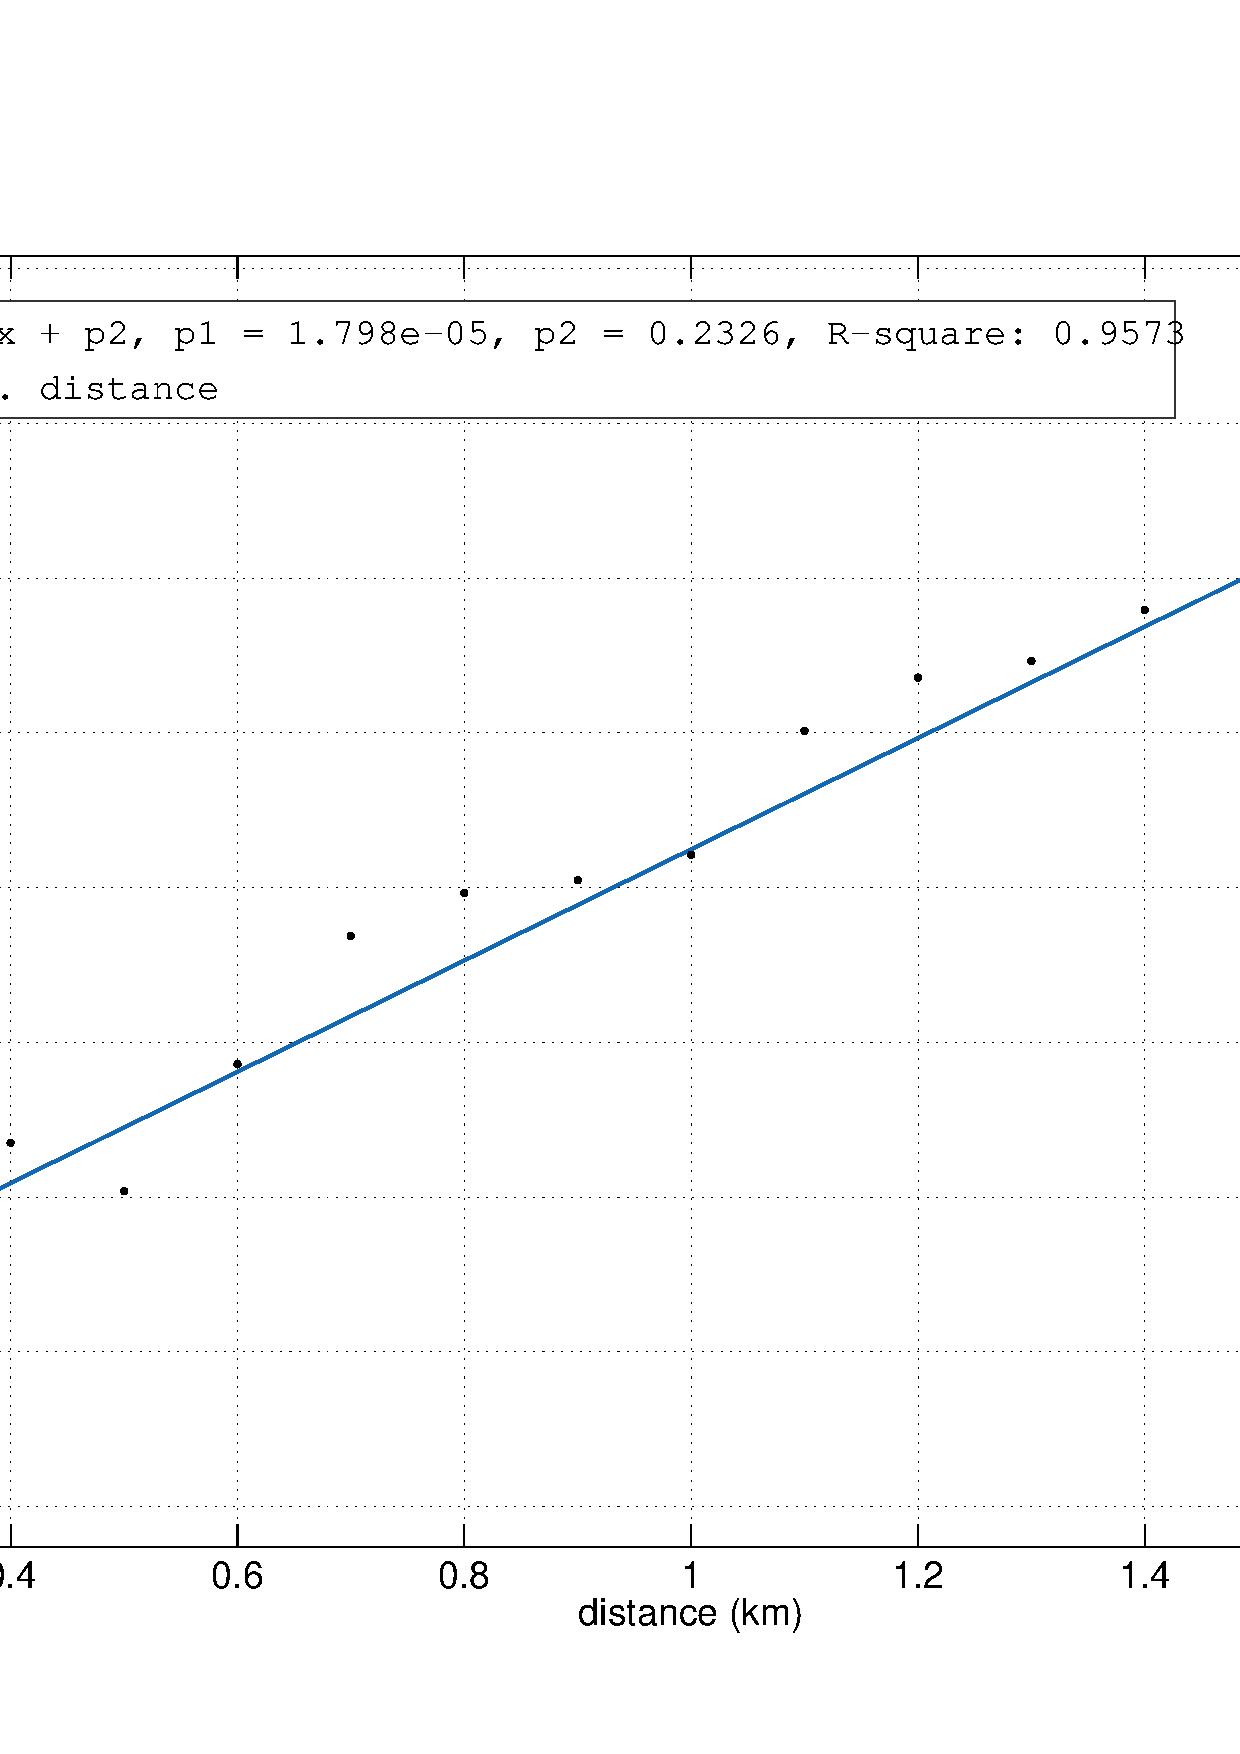
\includegraphics[width=\linewidth]{../figs/fit_curve.pdf}
  \vspace{-1em}
  \caption{Linear fitting of latency vs. distance}
  \label{fig:fit_curve}
\end{figure}

The gap between real latency performance and spped-of-light limit can be clearly observed, and identifying the source of the gap in current Internet remains our future work. 


%%% Local Variables: 
%%% mode: latex
%%% TeX-master: "main"
%%% End: 

\section{Latency for DC conversations}

\subsection{Methodology}

Bearing in mind that the primary goal for this part is to understand the partition of latency from end-users' perspective, we designed the experiment to perform data center related tasks. We expect the model in Fig.\,\ref{fig:DC_model} to be used, and the fractions in the WAN and the DC are also shown. 

\begin{figure}
  \centering
  \includegraphics[width=\linewidth]{../figs/DC_model.pdf}
  \caption{Typical user-DC communication pattern}
  \label{fig:DC_model}
\end{figure}

As an representative user-facing service, we have chosen Google Search as the case study. One of the reason of choosing Google Search is that they provide an estimated time spent within their DC (Fig.\,\ref{fig:google_time}). From our analysis in Sec.\,\ref{sec:analysis}, this data is fairly accurate in reflecting the fraction in DC. 

\begin{figure}
  \centering
  \includegraphics[width=0.85\linewidth]{../figs/GoogleTime.pdf}
  \caption{Google Search estimated time spent within Google in the return webpage}
  \label{fig:google_time}
\end{figure}

To measure the time for a single query, this can be easily done at the end-host side by timestamping the start and end of each query. But what to query remains a problem. Initially, we were suspecting that caching might happens at the Internet-facing router in DC. Querying the hottest words which are likely to be cached might reveal the WAN fraction. On the other side, to force the query to be processed by the DC (eliminating caching), we use random string for search. The hottest words can be found in Google Trends\footnote{http://www.google.com/trends/hottrends}, and we generate random strings comprised of lower cases, upper cases and numbers with length 32. Though the analysis in Sec.\,\ref{sec:analysis} shows a different results instead of what we have expected. This methodology is still useful to understand the problem we are initially planning to solve. 

In the meantime, {\it ping} is performed to measure the networking latency from the user to Google. Since we plan to conduct this experiment in geographically distributed fashion, and Google has many user-facing servers/IPs, we have to make sure we are measuring the right one. In this case, in additional to application layer HTTP conversation, we use {\it tcpdump} to capture all the packets and find out Google's IP address to ping.
 
In summary, to conduct the WAN vs. DC measurement, we issue query to Google and measure four different ``times'', shown in Table.\,\ref{tab:DC_method}.

\begin{table}
  \begin{tabular}{p{2.8cm} | p{5cm}}
    \hline
    type & description \\
    \hline
    Hot-trend-query time & the time spent to query a hot trend word to Google. \\
    Random-query time & the time spent to query a 32-character random string.  \\
    Ping time & the networking layer round-trip time to the responded Google IP address. \\
    Google time & Google's estimated time spent within their DC. \\
    \hline
  \end{tabular}
  \caption{Four different ``times'' measured}
  \label{tab:DC_method}
\end{table}

\subsection{Implementation and Experiement}
\label{sec:impl-exper}

We implement this measurement script in Python, and use {\it cron} to schedule the execution every two hours. Each time, the script will first visit Google Trends webpage and obtain the hot-trend words for that hour. Together with random generated strings, we obtain a list of 20 words for query. The entire list is queried for 10 times repeatedly, and four ``times'' are recorded. Each query is conducted using Python urllib2 library through HTTP, and the query address is ``http://www.google.com/search?hl=en\&output=search\&q=\%s"

% \begin{itemize}
% \setlength{\leftmargin}{-1pt}
% \setlength{\itemsep}{1pt}
% \setlength{\parskip}{0pt}
% \setlength{\parsep}{0pt}
% \item Hot-trend-query time \\
%   the time spent to query a hot trend word to Google. 
% \item Random-query time -- the time spent to query a 32-character random string. 
% \item Ping time -- the networking layer round-trip time to the responded Google IP address.
% \item Google time -- Google's estimated time spent within their DC.
% \end{itemize}

\subsection{Analysis}
\label{sec:analysis}

\begin{figure}
  \centering
  \includegraphics[width=\linewidth]{../figs/data_center.pdf}
  \caption{The latency measured in DC conversation experiments}
  \label{fig:data_center}
\end{figure}

%%% Local Variables: 
%%% mode: latex
%%% TeX-master: "main"
%%% End: 


\section{Latency within the Cellular Networks}

\subsection{Methodology}
\label{sec:methodology}


\subsection{Analysis}
\label{sec:analysis}

\begin{figure}
  \centering
  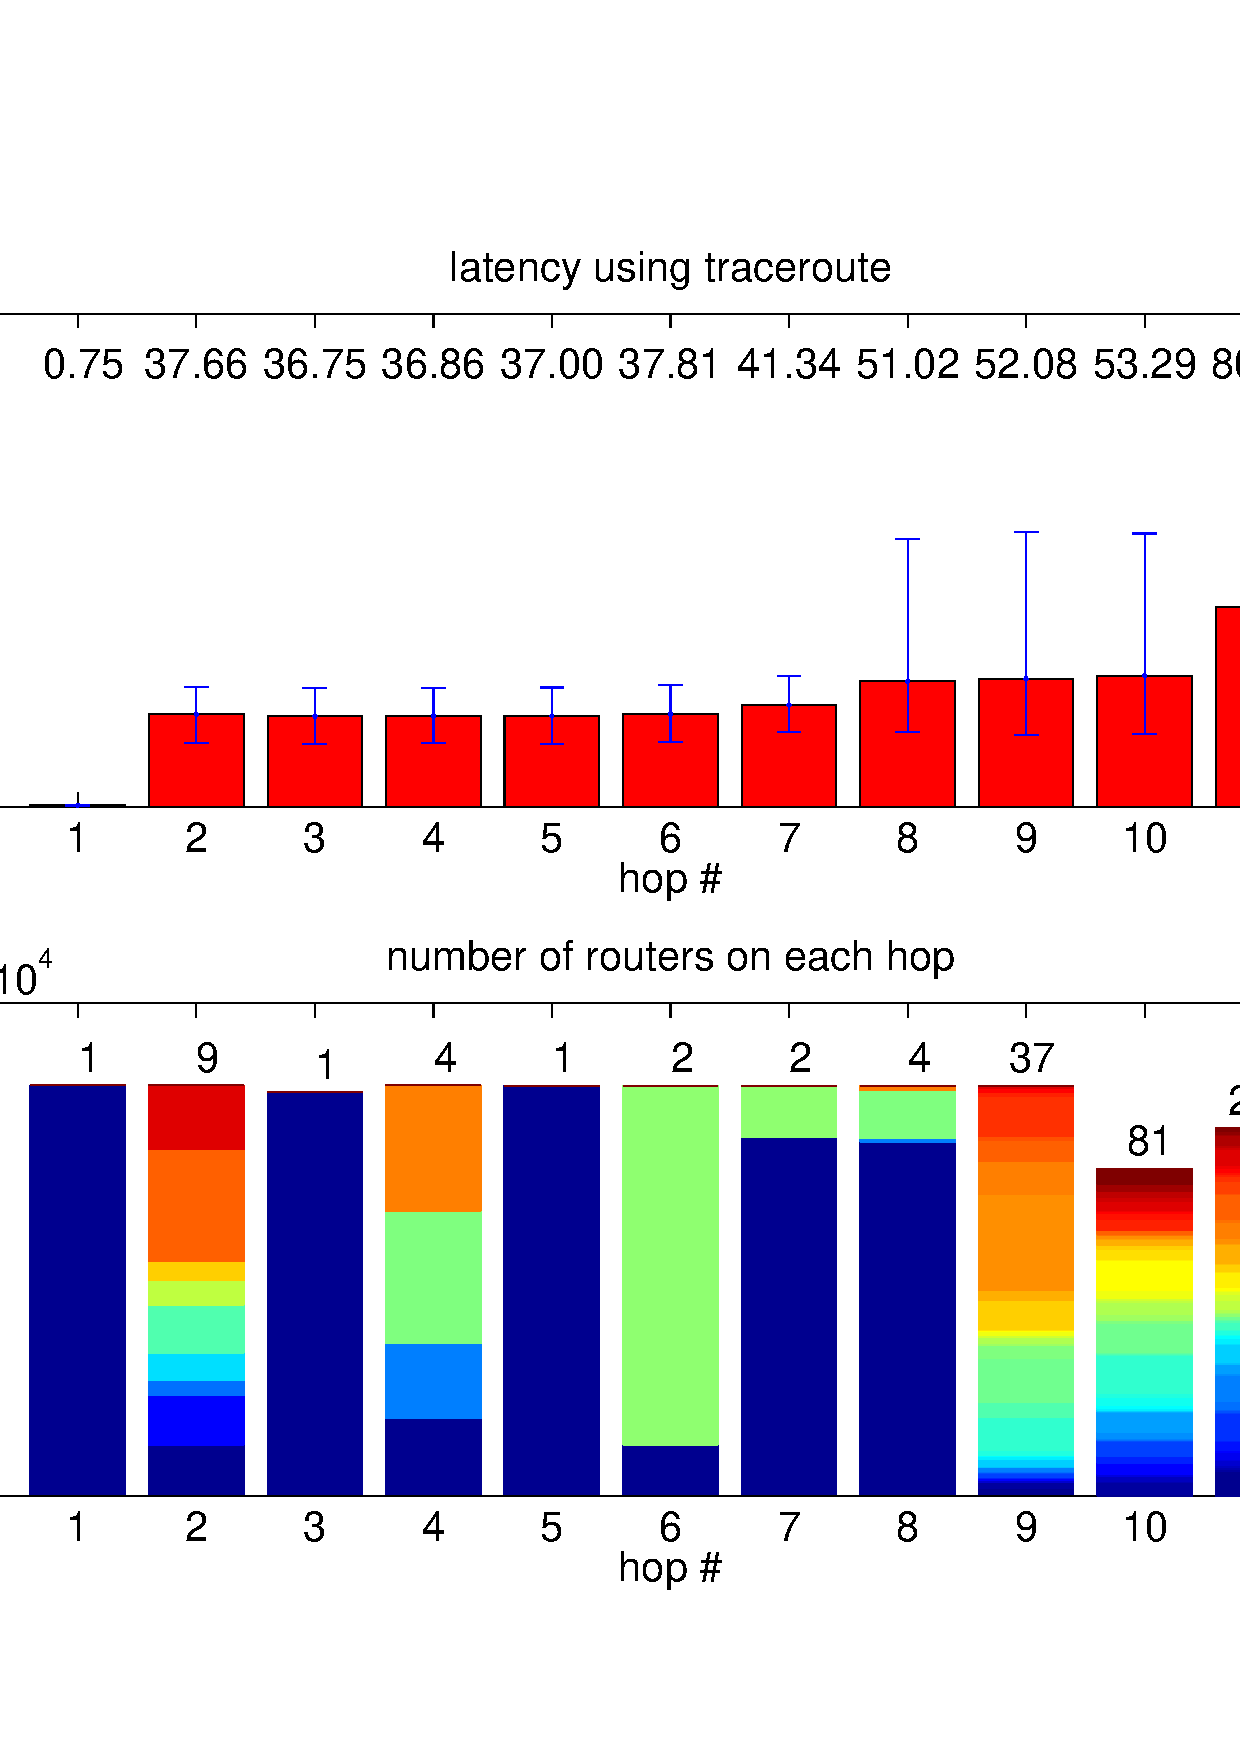
\includegraphics[width=\linewidth]{../figs/mobile_latency.pdf}
  \caption{Latency measured in each hop of AT\&T cellular networks}
  \label{fig:mobile_latency}
\end{figure}

\begin{figure}
  \centering
  \includegraphics[width=\linewidth]{../figs/routing_flaps.pdf}
  \caption{Routing flaps within AT\&T cellular networks}
  \label{fig:mobile_flaps}
\end{figure}

\begin{figure}
  \centering
  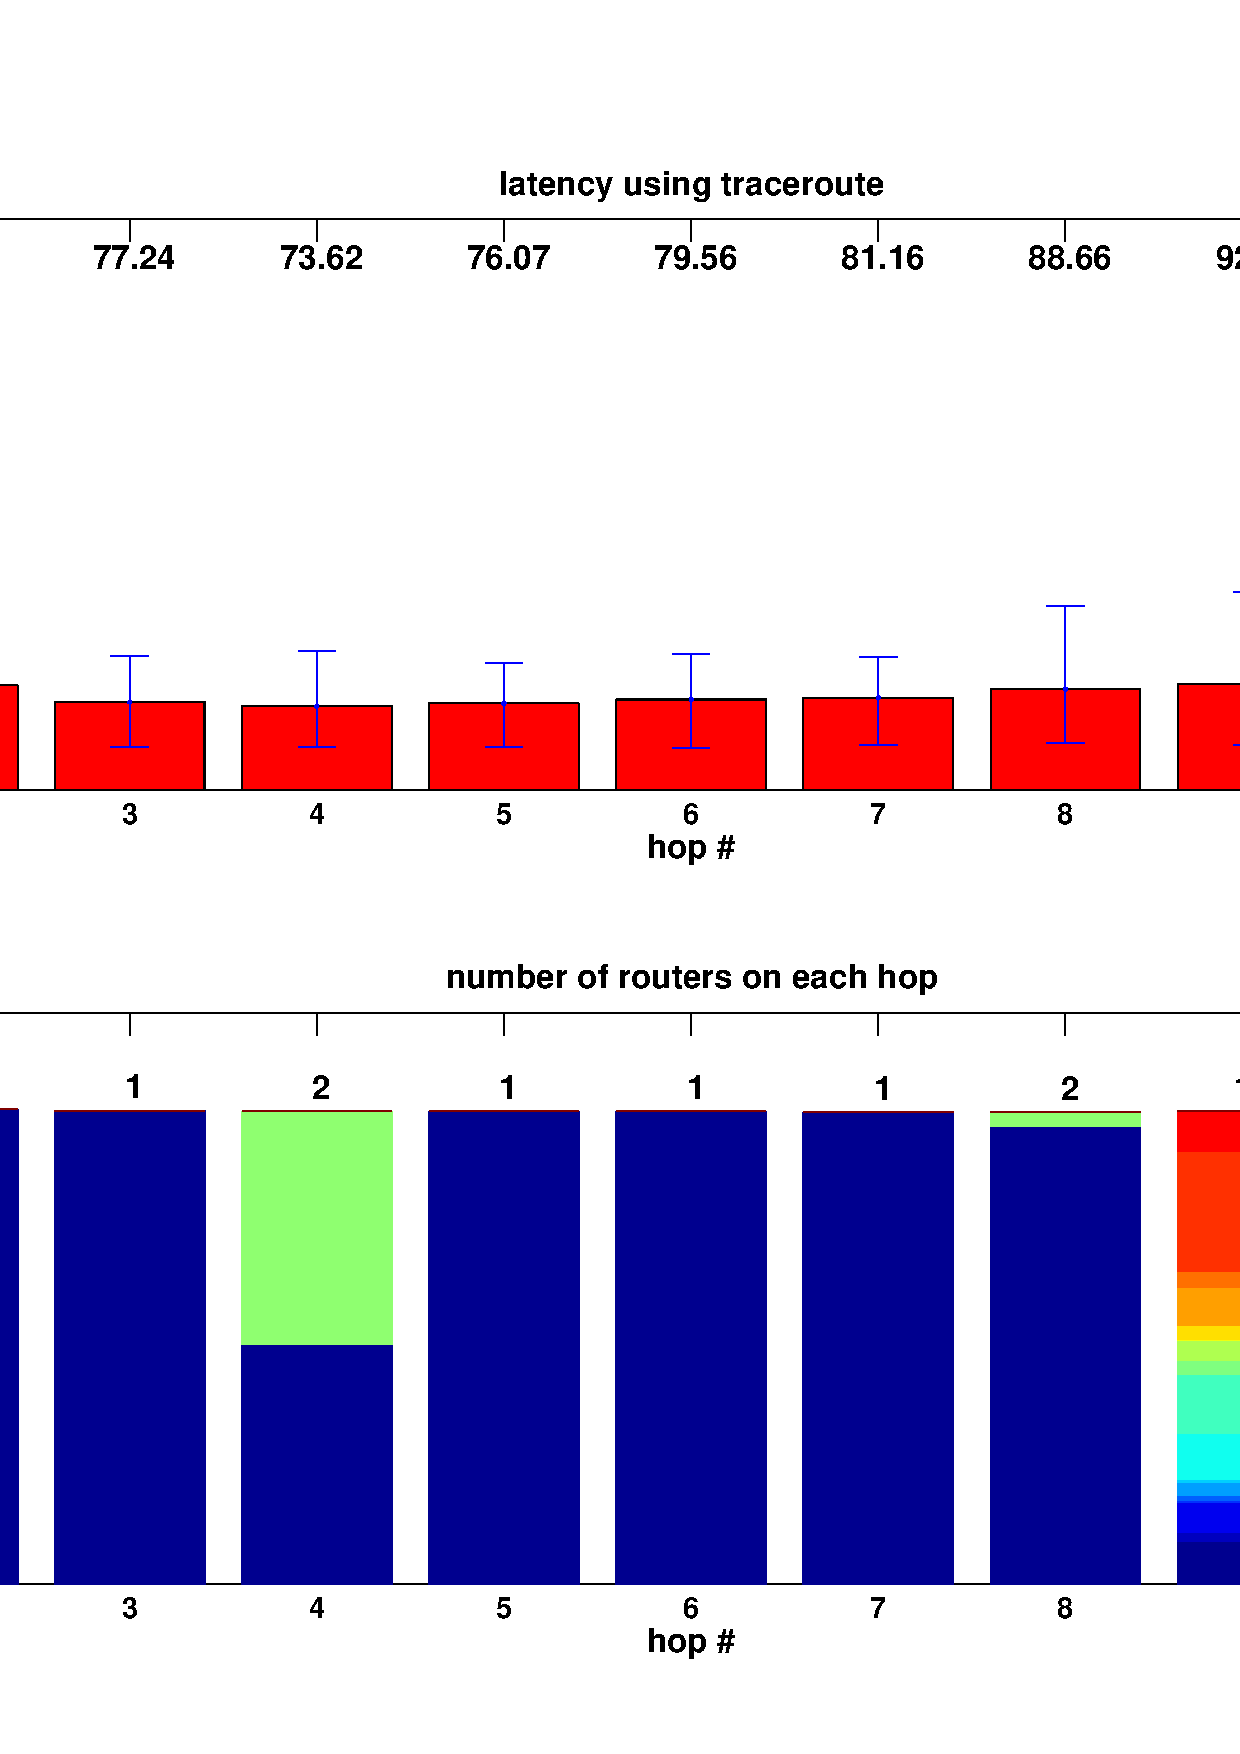
\includegraphics[width=\linewidth]{../figs/mobile_sfo.pdf}
  \caption{Latency when mobile phone is moving between Berkeley and San Francisco}
  \label{fig:mobile_mobile}
\end{figure}

%%% Local Variables: 
%%% mode: latex
%%% TeX-master: "main"
%%% End: 


\section{Discussion}
\label{sec:discussion}


%%% Local Variables: 
%%% mode: latex
%%% TeX-master: "main"
%%% End: 


\section{Conclusion and Future Work}
\label{sec:conclusion}

We believe that our results are relevant in displaying the current state of latency in wide-area, data center, and mobile networks. It is our goal to continue collecting measurements and refine our methodologies. Our next step is to compare our wide-area latency results to existing datasets, such as iPlane. For our DC measurements, we plan on re-evaluating our querying strategy; we hope to develop a better method of generating query strings as well as a long term solution to overcoming the limit on query rate. Finally, we hope to expand our mobile network study by measuring full application layer tasks, such as HTTP requests.

%%% Local Variables: 
%%% mode: latex
%%% TeX-master: "main"
%%% End: 


% \section{Acknowledgments}

\bibliographystyle{abbrv}
\bibliography{Measurement}

\end{document}